% =====================================================================
% AAI-501 Introduction to Artificial Intelligence
% Final Team Project - Group 2
% Phishing URL Detection on PhiUSIIL
%
% Build:  pdflatex main  ->  biber main  ->  pdflatex main  ->  pdflatex main
% Needs:  apa7, biblatex-apa (biber), booktabs, tabularx, listings, xcolor,
%         graphicx, csquotes, babel  (all standard in TeX Live / MacTeX)
% Figures expected in  ./figures/   Code expected in  ./code/
% =====================================================================
\documentclass[stu,12pt,floatsintext]{apa7}

\usepackage[american]{babel}
\usepackage{csquotes}
\usepackage[style=apa,sortcites=true,sorting=nyt,backend=biber]{biblatex}
\DeclareLanguageMapping{american}{american-apa}
\addbibresource{references.bib}

\usepackage{graphicx}
\usepackage{booktabs}
\usepackage{tabularx}
\usepackage{array}
\usepackage{setspace}      % ensures \singlespacing is defined for Appendix C
\usepackage{xcolor}
\usepackage{listings}

% left-ragged X column for wide tables (avoids underfull-hbox stretch)
\newcolumntype{Y}{>{\raggedright\arraybackslash}X}

% inline code helper (handles underscores etc. verbatim)
\newcommand{\code}[1]{\texttt{#1}}

% Python listing style for Appendix C
\definecolor{codegray}{gray}{0.5}
\definecolor{codekw}{rgb}{0.13,0.29,0.53}
\definecolor{codestr}{rgb}{0.16,0.50,0.16}
\definecolor{codecom}{rgb}{0.45,0.45,0.45}
\lstdefinestyle{py}{
  language=Python,
  basicstyle=\ttfamily\footnotesize,
  keywordstyle=\color{codekw}\bfseries,
  stringstyle=\color{codestr},
  commentstyle=\color{codecom}\itshape,
  numbers=left, numberstyle=\tiny\color{codegray}, numbersep=8pt,
  frame=single, rulecolor=\color{codegray!40},
  breaklines=true, breakatwhitespace=false,
  columns=fullflexible, keepspaces=true, showstringspaces=false,
  tabsize=4, xleftmargin=16pt,
  extendedchars=true, inputencoding=utf8,
  literate=%
    {↑}{{$\uparrow$}}1 {↓}{{$\downarrow$}}1
    {–}{{--}}1 {—}{{---}}1
    {“}{{``}}1 {”}{{''}}1 {‘}{{`}}1 {’}{{'}}1
    {≈}{{$\approx$}}1 {≤}{{$\leq$}}1 {≥}{{$\geq$}}1 {×}{{$\times$}}1,
}

% ------- Title page metadata (APA 7 student paper) -------------------
\title{Phishing URL Detection on PhiUSIIL: A Leakage-Aware Comparison of
Classical, Character-Level, and Clustering Methods}
\shorttitle{Phishing URL Detection on PhiUSIIL}
\author{Pranav Dhinakar, Jason Justice, and Guna Pasupathy}
\affiliation{Shiley-Marcos School of Engineering, University of San Diego}
\course{AAI-501: Introduction to Artificial Intelligence}
\professor{Professor [Instructor Name]}
\duedate{August 10, 2026}

\authornote{%
Group 2 final team project. Source code and full commit history are
available in the team GitHub repository:
\url{https://github.com/jjusticeusd/AAI-501-Final-Team-Project-Group2.git}.
A disclosure of generative-AI assistance appears in Appendix~B.}

\abstract{%
Phishing remains one of the most common vectors for scams and data
breaches, and automated URL classification is a practical application of
supervised learning. We build and evaluate a phishing-detection pipeline
on the PhiUSIIL Phishing URL Dataset (235{,}795 labeled URLs, 54
features) and organize the work around a single finding: on this
benchmark, near-perfect separability is intrinsic to the data rather than
an artifact of any one leaky column or train/test split. We audit the
dataset for leakage and confirm that content and lexical features reach
roughly 99.9\% accuracy with or without the obviously leaky
\code{URLSimilarityIndex}. We then compare three classical classifiers
(logistic regression, random forest, and XGBoost) with class-imbalance,
tuning, feature-importance, and cost-sensitive analyses; a character-level
convolutional network trained on the raw URL string alone as a
leakage-immune ``hard mode'' comparison; and an unsupervised clustering of
phishing rows into interpretable attack families. The character model
reaches 0.9985 accuracy and 0.9993 PR-AUC using only URL characters,
essentially tying the full-feature tabular models and demonstrating that
the separability lives in the URL strings themselves. All supervised
models land inside the published 99.5--100\% PhiUSIIL band. We therefore
frame the contribution not as a new accuracy ceiling but as an explanation
of why the ceiling exists and what kinds of phishing the benchmark
contains.}

\begin{document}
\maketitle

% =====================================================================
\section{Introduction}
% (Written for the report; ties the three notebooks together.)
% =====================================================================

Phishing is among the most common techniques used for scams and data
breaches, and automated detection of malicious web addresses is a
practical, high-impact application of supervised machine learning. This
project builds and evaluates a system that classifies a URL as phishing or
legitimate and, in doing so, compares more than one family of algorithms
under a controlled experimental design, as the course project requires.

We use the PhiUSIIL Phishing URL Dataset (UCI Machine Learning Repository,
id 967), which contains 235{,}795 labeled URLs described by 54 features.
The target column \code{label} encodes 1 for legitimate and 0 for
phishing. The dataset is large, has no missing values, and ships with
pre-engineered lexical and page-content features, so it satisfies the
project's size and preprocessing constraints without heavy cleaning.

The intellectual core of the project is a leakage-first framing. PhiUSIIL
is known to be ``too easy'' when every column is handed to a model, and a
naive report could stop at a near-perfect accuracy number. We instead
treat that near-perfection as the thing to be explained. Our central
finding, established three separate ways across the notebooks, is that the
separability of phishing from legitimate URLs is a property of the feature
set and even of the raw URL strings, not a side effect of one leaky
column or a favorable split. Every modeling result in this report is read
through that lens.

The work maps onto several topics from the course. It uses supervised
binary classification and ensemble methods (logistic regression, random
forest, and gradient boosting), feature selection and model-based feature
importance, and model evaluation under mild class imbalance (precision,
recall, F1, ROC-AUC, and PR-AUC). It connects to deep learning through a
character-level convolutional network applied to raw URL text, which also
touches the NLP idea of learning from character sequences. Finally it uses
unsupervised clustering (KMeans and HDBSCAN) to characterize structure
within the phishing class, satisfying the requirement to combine at least
two different algorithm types.

The report follows the three notebooks that make up the project code.
Section~2 presents the data audit and exploratory analysis (Notebook 01,
Guna Pasupathy), which establishes the leakage-clean feature set and split
conventions used everywhere else. Section~3 presents the classical models,
class-imbalance handling, tuning, feature importance, and a
cost-sensitive decision layer (Notebook 02, Jason Justice). Section~4
presents the grouping decision, the character-level model, the clustering
of attack families, and the state-of-the-art comparison (Notebook 03,
Pranav Dhinakar). Section~5 synthesizes the three notebooks against the
leakage thesis and the project requirements, and Section~6 concludes.

% =====================================================================
\section{Data, Leakage Audit, and Exploratory Analysis}
% Notebook 01 - Guna Pasupathy. Verbatim notes.
% =====================================================================

\emph{This section reproduces the analysis and commentary of Notebook 01
(author: Guna Pasupathy). The dataset is the PhiUSIIL Phishing URL Dataset
(UCI id 967): 235{,}795 URLs, 54 features, with \code{label} equal to 1
for legitimate and 0 for phishing. Because this dataset is known to be
``too easy'' if every column is thrown at a model, the notebook checks for
data leakage before any modeling: it loads the data, looks at class
balance and duplicates, checks the leaky and suspicious columns
(\code{URLSimilarityIndex}, too-perfect yes/no features, repeated domains,
\code{TLD}), and saves the list of safe feature columns for Notebooks 02
and 03.}

There are no missing values at all, which matches the UCI description. The
four string columns are \code{URL}, \code{Domain}, \code{TLD}, and
\code{Title}.

\subsection{Class Balance}

About 57\% of the rows are legitimate and 43\% are phishing
(Figure~\ref{fig:class-balance}). The proposal feedback assumed a heavily
imbalanced dataset, but this is only a mild imbalance, so aggressive
resampling is not needed. The plan is to use class weights in the models
and to try SMOTE only as a comparison experiment (Notebook 02).

\begin{figure}[htbp]
\centering
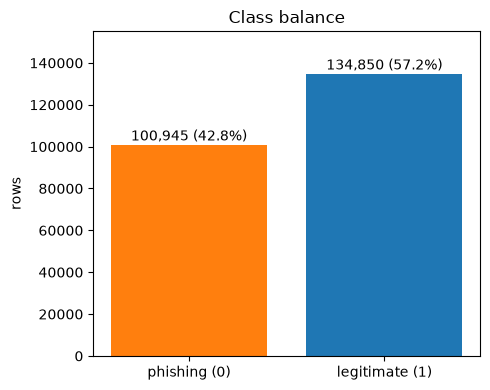
\includegraphics[width=0.5\linewidth]{figures/fig_class_balance.png}
\caption{Class balance in PhiUSIIL. Legitimate URLs (label 1) slightly
outnumber phishing URLs (label 0), a roughly 57/43 split.}
\label{fig:class-balance}
\end{figure}

\subsection{Duplicate Rows and Duplicate URLs}

There are no fully duplicated rows, but 425 URLs appear more than once
(always with the same label). If the same URL lands in both train and
test, the model gets tested on something it literally saw during training.
Notebook 02 therefore drops duplicate URLs before splitting.

\subsection{Leakage Check 1: \texorpdfstring{\code{URLSimilarityIndex}}{URLSimilarityIndex}}

This column measures how similar a URL is to known legitimate URLs, so it
basically contains the answer. Every single legitimate URL scores exactly
100 (standard deviation 0), which is clearly leakage. It is not perfect in
the other direction though: 786 phishing URLs also score 100, so the
column alone cannot reach 100\% accuracy (Figure~\ref{fig:urlsim}). The
log scale is needed because the legitimate spike at 100 (134{,}850 rows)
would otherwise flatten the phishing distribution.

\begin{figure}[htbp]
\centering
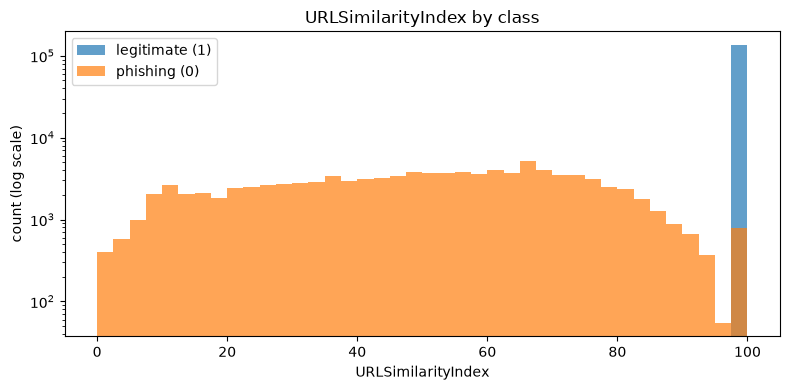
\includegraphics[width=0.8\linewidth]{figures/fig_urlsimilarity_hist.png}
\caption{Distribution of \code{URLSimilarityIndex} by class (log-scaled
counts). Legitimate URLs pile up at exactly 100; a minority of phishing
URLs also reach 100.}
\label{fig:urlsim}
\end{figure}

How much does this one column matter? A quick logistic regression shows
the leaky column alone gets 99.6\%. But here is the surprise: dropping it
barely matters, because the remaining roughly 50 features together get
99.9\%. So the dataset is almost trivially easy even without the leaky
column. That makes sense (features like \code{HasPasswordField} or
\code{LineOfCode} come from crawling the actual page), but it means the
tabular models solve an easy version of the problem. That is why the plan
also includes a model that only sees the raw URL string (Notebook 03),
which is the honest ``hard mode'' result.

\subsection{Leakage Check 2: Too-Perfect Yes/No Features}

If one class almost always has a flag and the other almost never does,
that smells like an artifact of how the dataset was collected rather than
a real-world rule. The standout is \code{IsHTTPS}: 100\% of legitimate
URLs use HTTPS, with zero exceptions, while about half the phishing URLs
do too. A rule ``no HTTPS = phishing'' would never be wrong on this
dataset, which is not true of the real web; it is a side effect of where
the legitimate URLs were collected. \code{HasSocialNet},
\code{HasCopyrightInfo}, and \code{HasDescription} have huge gaps too
(real sites have footers and meta tags, parked phishing pages usually do
not). Dropping the top six giveaway flags (including \code{IsHTTPS}) and
re-running the quick model barely changes accuracy. The easiness is spread
across the whole feature set, not hidden in a few columns, so there is no
clean line where we could keep ``some'' content features and get an honest
problem. Decision: keep these features for the tabular models
(Notebook 02) but call out \code{IsHTTPS} and friends in the report as
collection artifacts, and treat the URL-only model in Notebook 03 as the
realistic difficulty level.

\subsection{Leakage Check 3: Repeated Domains}

\code{URL} and \code{Domain} are basically IDs, so they stay out of the
feature set either way. But if the same domain shows up in both train and
test, the model can memorize the domain instead of learning patterns.
About 9\% of rows share a domain with another row. The top of the list is
telling: \code{ipfs.io}, \code{gateway.ipfs.io}, \code{cloudflare-ipfs.com}
and \code{cf-ipfs.com} are all gateways to the same IPFS service, so exact
string matching actually \emph{under}-counts how related the rows are.
Being stricter would mean grouping by registered domain (for example with
the \code{tldextract} package), which Notebook 03 revisits. Comparing a
normal random split against a split that keeps each domain on one side
only shows essentially no difference: the score was not inflated by
repeated domains, the dataset is just this easy. Still, the grouped split
is the safer choice and costs nothing, so Notebook 02 uses
\code{GroupShuffleSplit} on \code{Domain} and reports both.

\subsection{The \texorpdfstring{\code{TLD}}{TLD} Column}

Two findings. First, 695 unique TLDs is too many to one-hot encode.
Second, 599 of them are not TLDs at all: for URLs that use a raw IP
address, whoever built the dataset took the last number of the IP as the
``TLD'' (for example, domain \code{198.98.58.123} gets TLD \code{123}).
All 599 of those rows are phishing. \code{IsDomainIP} already captures this
signal, so it is a data-quality quirk to mention, not something to fix.
Instead of encoding \code{TLD} the plan is to use \code{TLDLegitimateProb},
a provided score for how trustworthy the TLD is. One worry: if UCI
computed that score \emph{from this dataset's own labels}, it would be
target leakage just like \code{URLSimilarityIndex}. If the score had been
computed from these labels, its correlation with the per-TLD share of
legitimate rows would be close to 1; at about 0.18 it clearly was not, so
it is fine to keep as a feature.

\subsection{Which Safe Features Correlate with the Label?}

The strongest safe features are mostly page-content ones
(\code{HasSocialNet}, \code{HasCopyrightInfo}, \code{IsHTTPS}, and so on),
matching the leakage-check results above (Figure~\ref{fig:label-corr}).
One caveat: plain correlation understates skewed count features like
\code{LineOfCode} or \code{NoOfImage}, so the notebook relies on
model-based feature importance in Notebook 02 rather than this chart for
feature selection.

\begin{figure}[htbp]
\centering
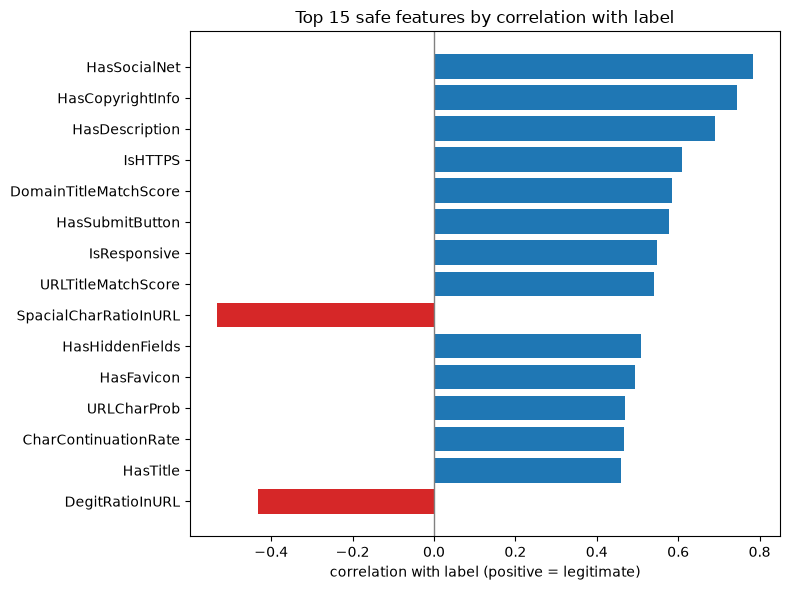
\includegraphics[width=0.8\linewidth]{figures/fig_label_correlations.png}
\caption{Top 15 safe features by absolute correlation with the label.
Page-content indicators dominate; blue is positive and red is negative
correlation.}
\label{fig:label-corr}
\end{figure}

\subsection{A Closer Look at Individual Features}

Everything above was about leakage. A normal EDA question is how the
features actually differ between the two classes. The page-content
features are the dramatic ones: the median phishing page has 12 lines of
code, zero JS files, zero images, and zero external references, while the
median legitimate page has over 1{,}100 lines of code. Most phishing pages
are basically empty shells. The URL-shape differences are real but much
smaller: phishing URLs are a bit longer and use more special characters.
Figure~\ref{fig:feat-dist} shows distributions for a few representative
features (top row = URL features, bottom row = page-content features).
The content features (bottom row) separate the classes almost by
themselves, with phishing piling up at zero, while the URL-shape features
(top row) overlap a lot. This is another preview of why the URL-only model
in Notebook 03 faces the harder problem.

\begin{figure}[htbp]
\centering
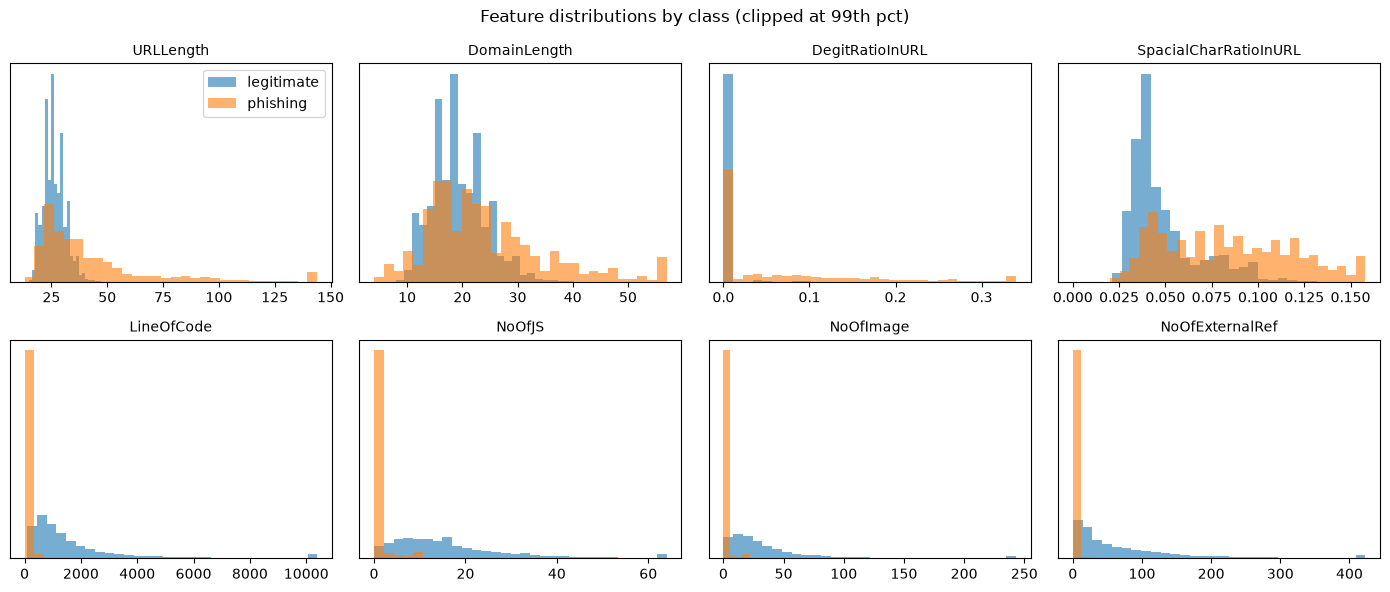
\includegraphics[width=\linewidth]{figures/fig_feature_distributions.png}
\caption{Per-class distributions (clipped at the 99th percentile) for
representative URL-shape features (top) and page-content features
(bottom). Phishing pages concentrate at zero on the content features.}
\label{fig:feat-dist}
\end{figure}

\subsection{Do Any Features Duplicate Each Other?}

A lot of columns look like counts and ratios of the same thing. Strongly
correlated features make logistic-regression coefficients hard to read and
are a known risk for the SMOTE experiment. There is less redundancy than
expected: only four pairs above an absolute correlation of 0.8, and only
two near-duplicates (\code{DomainTitleMatchScore} / \code{URLTitleMatchScore}
and \code{URLLength} / \code{NoOfLettersInURL}). Nothing so extreme that
features need to be dropped up front. The heatmap
(Figure~\ref{fig:corr-heatmap}) does show the strongest features are
moderately correlated with each other; they all measure some version of
``does this page have real content.'' So when Notebook 02 looks at feature
importance, credit may be split between similar features and exact
rankings should not be over-interpreted.

\begin{figure}[htbp]
\centering
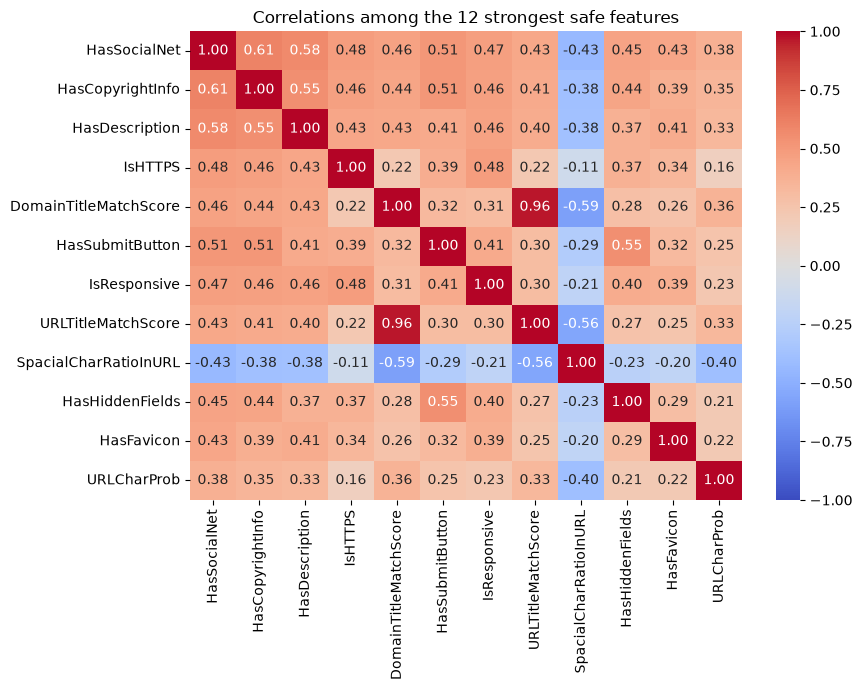
\includegraphics[width=0.75\linewidth]{figures/fig_correlation_heatmap.png}
\caption{Correlation heatmap among the twelve features most correlated
with the label. The strong content features are moderately
inter-correlated.}
\label{fig:corr-heatmap}
\end{figure}

\subsection{Summary of the Data Audit}

The audit establishes the following, all of which shape the modeling in
Notebooks 02 and 03:

\begin{itemize}
  \item \textbf{Class balance is mild} (57/43), not severe. Class weights
    first, SMOTE only as a comparison.
  \item \textbf{\code{URLSimilarityIndex} is leaky} (every legitimate row
    equals 100) and is dropped, but the other features still reach roughly
    99.9\%, so the dataset is easy with or without it. The URL-string-only
    model in Notebook 03 is the realistic-difficulty comparison.
  \item \textbf{\code{IsHTTPS} is a collection artifact} (100\% of
    legitimate rows are HTTPS). It is kept but flagged; dropping the top
    giveaway flags barely changes accuracy.
  \item \textbf{425 duplicate URLs} lead Notebook 02 to drop URL
    duplicates before splitting.
  \item \textbf{9\% of rows share a domain}, so Notebook 02 uses a
    domain-grouped split. The quick check says it does not change the
    score, but it is the safer setup.
  \item \textbf{599 IP-address rows have junk numeric ``TLDs''} (all
    phishing), a data-quality quirk worth a sentence in the report.
  \item \textbf{\code{TLDLegitimateProb} checks out as non-leaky}
    (correlation about 0.18 with the labels), so it is used instead of
    one-hot encoding 695 TLDs.
  \item \textbf{Phishing pages are empty shells}: median 12 lines of code
    and zero JS/images/external references, versus 1{,}105 lines of code
    for the median legitimate page. URL-shape features overlap far more
    between the classes.
  \item \textbf{Feature redundancy is mild} (only four pairs with absolute
    correlation above 0.8), but the strong content features are moderately
    inter-correlated, so feature-importance rankings in Notebook 02 should
    not be over-interpreted.
\end{itemize}

The safe feature list is saved to \code{data/01\_feature\_columns.json} so
the other notebooks all use the same agreed feature set.

% =====================================================================
\section{Classical Models}
% Notebook 02 - Jason Justice. Verbatim notes.
% =====================================================================

\emph{This section reproduces the modeling and commentary of Notebook 02
(author: Jason Justice). Building on Notebook 01's leakage-clean feature
list, it (1) engineers new features from the raw URL/Domain strings, (2)
trains three classifiers on the clean feature set, (3) handles the mild
class imbalance and tests whether SMOTE helps, (4) tunes the strongest
model and reads off feature importance, (5) checks whether a handful of
top features match the full model, and (6) adds a cost-sensitive decision
layer.} An important note on label orientation: the raw \code{label} is 1
for legitimate and 0 for phishing, and this notebook models \textbf{phishing
as the positive class} (\code{y = 1 - label}) so that precision, recall,
and PR-AUC all describe \emph{catching phishing}.

\subsection{Engineered Features}

PhiUSIIL already ships lexical ratios and page-content counts. To add
something genuinely new, the notebook builds four signals from the raw
\code{URL} / \code{Domain} strings (held out of the clean set as
identifiers) that those columns do not already encode:

\begin{itemize}
  \item \textbf{\code{url\_entropy} / \code{domain\_entropy}}:
    character-level Shannon entropy. Randomly generated (DGA-style)
    domains tend to look more random.
  \item \textbf{\code{brand\_distance}}: the smallest normalized edit
    distance from any significant domain label to a curated brand list. A
    domain that is \emph{close but not equal} to a known brand is the
    classic typosquatting signal (for example, \code{paypa1},
    \code{paypal-secure}).
  \item \textbf{\code{is\_punycode}}: the domain uses \code{xn--} (IDN
    homograph attacks).
  \item \textbf{\code{is\_shortener}}: the registered domain is a known URL
    shortener.
\end{itemize}

A quick look before modeling (medians by class and the distributions of
the three continuous features) appears in
Figure~\ref{fig:engineered-dist}.

\begin{figure}[htbp]
\centering
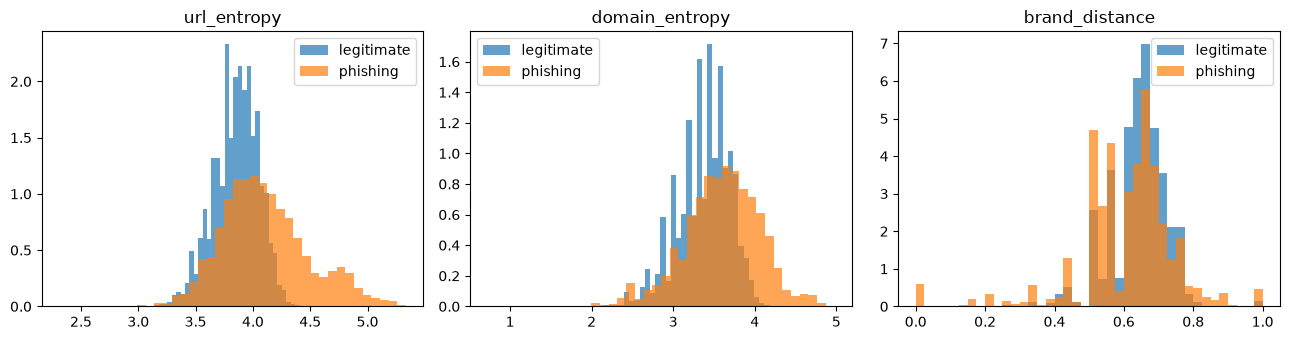
\includegraphics[width=0.9\linewidth]{figures/fig_engineered_distributions.png}
\caption{Distributions of the engineered continuous features by class.
Class separation is modest, foreshadowing their low importance once the
shipped content features are present.}
\label{fig:engineered-dist}
\end{figure}

\subsection{Assembling the Modeling Frame}

Following Notebook 01's manifest, the notebook drops duplicate URLs (so
the same URL cannot land in both train and test), models phishing as the
positive class, and splits with a domain-grouped 80/20 split so every row
of a domain stays on one side.

\subsection{Model Roster}

Three classifiers are used, all treating phishing as the positive class:
logistic regression (class-weighted) as an interpretable linear baseline;
random forest (class-weighted) for a non-linear model with feature
importance; and XGBoost (\code{scale\_pos\_weight}) as the strongest
tabular model. The notebook reports accuracy, precision, recall, F1,
ROC-AUC, and PR-AUC (\code{average\_precision}), the last being the more
informative summary under class imbalance. Results are in
Table~\ref{tab:roster}; confusion matrices are in
Figure~\ref{fig:conf-classical}.

\begin{table}[htbp]
\centering
\caption{Classical model performance on the shared test set
(phishing = positive class).}
\label{tab:roster}
\begin{tabular}{lcccccc}
\toprule
Model & Accuracy & Precision & Recall & F1 & ROC-AUC & PR-AUC \\
\midrule
Logistic Regression & 0.9995 & 0.9995 & 0.9993 & 0.9994 & 1.0 & 1.0 \\
Random Forest       & 0.9999 & 0.9999 & 0.9998 & 0.9999 & 1.0 & 1.0 \\
XGBoost             & 0.9999 & 1.0000 & 0.9998 & 0.9999 & 1.0 & 1.0 \\
\bottomrule
\end{tabular}
\end{table}

\begin{figure}[htbp]
\centering
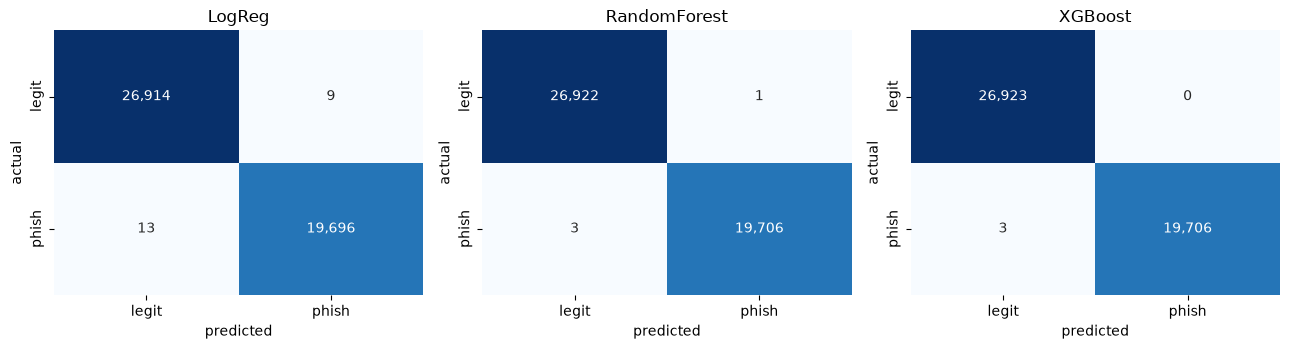
\includegraphics[width=\linewidth]{figures/fig_confusion_classical.png}
\caption{Confusion matrices for the three classifiers. Rows are the true
class, columns the prediction, with phishing as the class of interest.}
\label{fig:conf-classical}
\end{figure}

\subsection{Class-Imbalance Handling}

The imbalance here is mild (about 57/43), so the notebook starts with the
cheap option, \code{scale\_pos\_weight}, and treats SMOTE as an explicit
ablation rather than a default. Three setups are compared on the same
XGBoost model: no balancing, class weighting, and SMOTE oversampling
(Table~\ref{tab:imbalance}). The three rows are nearly identical: on mild
imbalance with an already-separable feature set, resampling buys
essentially nothing (and SMOTE synthesizes points among correlated tabular
features, a known overfitting risk). The notebook keeps
\code{scale\_pos\_weight} as the cheap default.

\begin{table}[htbp]
\centering
\caption{Imbalance-handling ablation on XGBoost.}
\label{tab:imbalance}
\begin{tabular}{lcccccc}
\toprule
Setup & Accuracy & Precision & Recall & F1 & ROC-AUC & PR-AUC \\
\midrule
none              & 0.9999 & 1.0 & 0.9998 & 0.9999 & 1.0 & 1.0 \\
scale\_pos\_weight & 0.9999 & 1.0 & 0.9998 & 0.9999 & 1.0 & 1.0 \\
SMOTE             & 1.0000 & 1.0 & 0.9999 & 0.9999 & 1.0 & 1.0 \\
\bottomrule
\end{tabular}
\end{table}

\subsection{Tuning the Strongest Model}

\code{RandomizedSearchCV} over XGBoost is scored on PR-AUC
(\code{average\_precision}) and cross-validated with
\code{StratifiedGroupKFold} so domains never straddle a fold boundary
during tuning either.

\subsection{Feature Importance}

The notebook uses two views: XGBoost's built-in gain importance
(Figure~\ref{fig:importance}) and model-agnostic permutation importance
(the drop in PR-AUC when a feature is shuffled), computed on a test-set
sample. It specifically checks where the four engineered features land.

\begin{figure}[htbp]
\centering
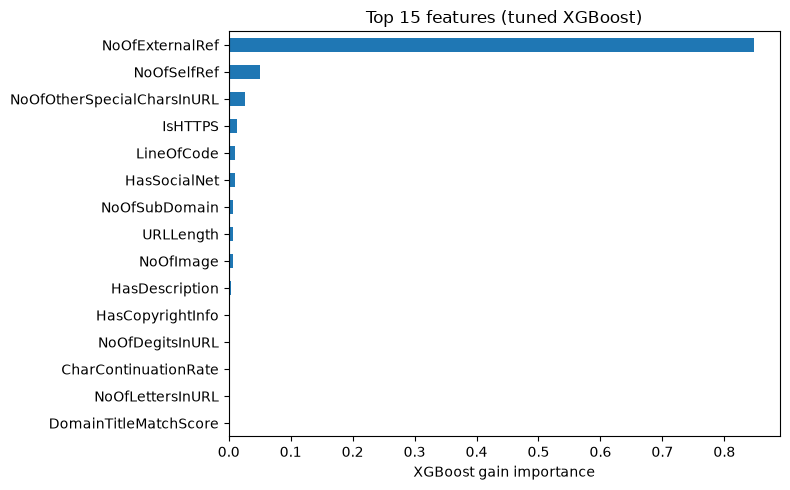
\includegraphics[width=0.8\linewidth]{figures/fig_feature_importance.png}
\caption{Top-15 XGBoost gain importances. Page-content and URL-structure
columns dominate; the four engineered features do not appear in the top
ranks.}
\label{fig:importance}
\end{figure}

\subsection{Does a Handful of Features Match the Full Model?}

The assignment calls out this pattern as the model of a good result: if a
model using only the top-K features nearly matches the full model, that is
an actionable finding, because a production filter could collect far fewer
signals per URL. Retraining XGBoost on just the top eight features
(\code{NoOfExternalRef}, \code{NoOfSelfRef},
\code{NoOfOtherSpecialCharsInURL}, \code{IsHTTPS}, \code{LineOfCode},
\code{HasSocialNet}, \code{NoOfSubDomain}, \code{URLLength}) nearly matches
the tuned full model (Table~\ref{tab:topk}).

\begin{table}[htbp]
\centering
\caption{Full tuned model versus a top-8-feature model.}
\label{tab:topk}
\begin{tabular}{lcccccc}
\toprule
Model & Accuracy & Precision & Recall & F1 & ROC-AUC & PR-AUC \\
\midrule
XGBoost (tuned)  & 0.9999 & 1.000 & 0.9998 & 0.9999 & 1.0 & 1.0 \\
XGBoost (top 8)  & 0.9994 & 0.999 & 0.9995 & 0.9993 & 1.0 & 1.0 \\
\bottomrule
\end{tabular}
\end{table}

\subsection{Cost-Sensitive Decision Layer}

Accuracy near the ceiling hides the real design question: where do you
want the few remaining errors to fall? That depends on the cost of each
error type, which is asymmetric for phishing. A false negative (phishing
let through) risks credential theft or fraud, so its cost is set an order
of magnitude higher, anchored loosely to public breach-cost figures. A
false positive (legitimate site blocked) costs user friction and support
load, an illustrative estimate rather than a sourced figure. Sweeping the
decision threshold and picking the operating point that minimizes expected
cost per 1{,}000 URLs (Figure~\ref{fig:cost}) yields a minimum-cost
threshold of 0.24, at \$21.44 per 1{,}000 URLs, versus \$32.17 at the
default threshold of 0.5.

\begin{figure}[htbp]
\centering
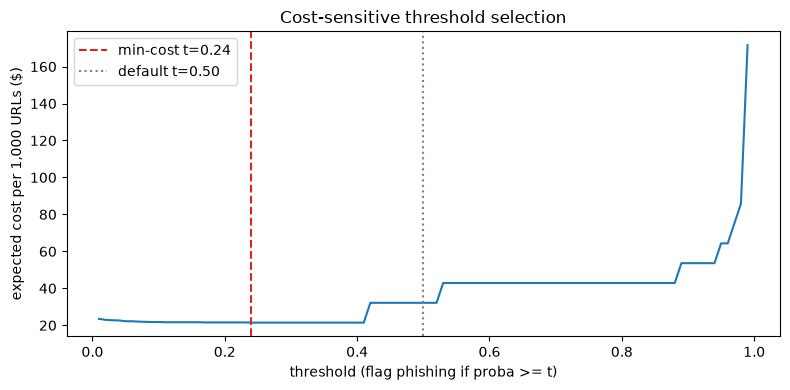
\includegraphics[width=0.7\linewidth]{figures/fig_cost_curve.png}
\caption{Expected cost per 1{,}000 URLs as a function of decision
threshold. The minimum sits at 0.24, below the default 0.5, reflecting the
higher cost assigned to false negatives.}
\label{fig:cost}
\end{figure}

\subsection{Business Metric: It Depends on the Deployment}

There is no single ``right'' metric; it follows the deployment scenario. A
browser warning system (Google Safe Browsing style) is precision-first,
because wrongly blocking a legitimate site is highly visible, so it accepts
lower recall for very high precision. A mail or endpoint gateway that
quarantines silently is recall-first, because a missed phishing email
reaching an inbox is the expensive outcome. The notebook reports both
operating points plus a three-tier allow/warn/block policy, which is closer
to how real filters behave than one binary cutoff: a precision-first point
at threshold 0.000 (precision 0.9900, recall 1.0000), a recall-first point
at threshold 0.412 (precision 1.0000, recall 0.9999), and a three-tier
policy that, on the test set, allows 26{,}926 URLs, blocks 19{,}704, and
warns on 2.

\subsection{Summary and Hand-Off}

\begin{itemize}
  \item \textbf{The engineered features barely move the needle here}: they
    land at the bottom of the importance ranking (ranks 22--54, about zero
    gain) and their by-class medians overlap heavily. That is itself an
    honest result. The shipped page-content columns (\code{IsHTTPS},
    \code{LineOfCode}, \code{NoOfExternalRef}, and so on) already carry
    essentially all the separating signal, so lexical entropy and
    brand-distance add little \emph{on top of them}. They may still earn
    their keep in the URL-only regime (Notebook 03), where those content
    columns do not exist.
  \item \textbf{Mild imbalance needs only class weighting}; SMOTE added
    nothing here and risks overfitting correlated tabular features.
  \item \textbf{The problem is near-saturated on tabular features} (about
    99.9\%, matching Notebook 01 and the published PhiUSIIL numbers), so
    the interesting work is what to do with the tiny error budget: the
    cost-sensitive layer and the precision-first versus recall-first
    operating points make that an explicit, business-driven choice rather
    than a default 0.5.
  \item \textbf{A top-8-feature model nearly matches the full model}, an
    actionable result for a cheaper production filter.
\end{itemize}

The harder, more honest difficulty regime, a model that never sees the
engineered or content features, is Notebook 03's character-level model on
the raw URL string, alongside the clustering and the full state-of-the-art
comparison.

% =====================================================================
\section{Character-Level Model, Clustering, and State of the Art}
% Notebook 03 - Pranav Dhinakar. Verbatim notes.
% =====================================================================

\emph{This section reproduces Notebook 03 (author: Pranav Dhinakar).
Following Notebook 02, phishing is modeled as the positive class so
precision, recall, and PR-AUC describe catching phishing. Notebook 01
established the leakage-clean feature set and split conventions, and
Notebook 02 built the tabular models and saved their metrics. This
notebook (1) settles the train/test grouping convention and locks it to
Notebook 02's for comparability, (2) trains a character-level CNN on the
raw URL string only as the leakage-immune ``hard mode'' comparison, (3)
clusters the phishing rows into attack ``families,'' and (4) assembles the
state-of-the-art comparison table.}

\subsection{Registered-Domain Grouping Decision}

Notebook 01 split on the exact \code{Domain} string and flagged that this
\emph{under}-groups subdomains: \code{ipfs.io}, \code{gateway.ipfs.io} and
\code{cf-ipfs.com} are the same service but count as three domains, so
related rows can still land on both sides of a train/test split. The
stricter alternative groups by registered domain (eTLD+1 via
\code{tldextract}), which collapses those into one group. This matters
because the character model, the clustering, and Notebook 02's tabular
models must all use the \emph{same} split, or the SOTA table compares
numbers produced under different conditions. Three grouping strictnesses,
run through the same quick logistic model, give the results in
Table~\ref{tab:grouping}.

\begin{table}[htbp]
\centering
\caption{Effect of grouping strictness on a quick logistic-regression
score.}
\label{tab:grouping}
\begin{tabular}{lccc}
\toprule
Grouping & Groups & Accuracy & F1 \\
\midrule
exact \code{Domain} (NB 01 / NB 02)     & 220{,}086 & 0.9995 & 0.9996 \\
PaaS-aware eTLD+1 (PSL-private on)       & 197{,}709 & 0.9993 & 0.9994 \\
naive eTLD+1                             & 175{,}509 & 0.9990 & 0.9992 \\
\bottomrule
\end{tabular}
\end{table}

Accuracy is essentially invariant (0.9990--0.9995) across a 44{,}577-group
range of strictness. The drop is monotonic with strictness, the direction
leakage would predict, but negligible in size, reinforcing Notebook 01's
finding that the dataset is easy regardless of how conservatively the
split is drawn. Because the score is grouping-invariant, the notebook
\textbf{adopts Notebook 02's exact \code{Domain} grouping}
(\code{GroupShuffleSplit}, \code{test\_size=0.2}, \code{random\_state=42})
rather than reworking it. This makes the character model share Notebook
02's exact test set, so the SOTA table compares numbers produced under
identical conditions. The stricter registered-domain analysis is retained
as evidence that this choice does not inflate the results.

\subsection{Character-Level Model on the Raw URL}

The tabular models in Notebook 02 use page-content and lexical features
that make PhiUSIIL trivially easy (about 99.9\%). This model sees only the
raw URL string: no engineered features, no page content, no
\code{URLSimilarityIndex}. It cannot leak, because it has access to
nothing but the characters of the URL itself, so it is the leakage-immune
comparison point for the URL-only lexical literature
(\textcite{sahingoz2019} reached 97.98\% with an NLP-feature random
forest). Each URL is tokenized at the character level, embedded, and
passed through a small 1-D CNN with a sigmoid output, trained with class
weights on the same exact-\code{Domain} split used in Notebook 02 so the
numbers are comparable.

\subsubsection{Architecture}

The model is a compact character-level CNN (\textcite{kim2014}, adapted to
characters). An embedding maps each character id to a 48-dimensional
vector (\code{padding\_idx=0}). Three parallel 1-D convolutions of kernel
widths 3, 5, and 7 (128 filters each) read character 3-, 5-, and 7-grams.
A global max-pool over position is followed by concatenation of the three
widths, dropout (0.4), a linear layer, and a single logit. The loss is
\code{BCEWithLogitsLoss} with \code{pos\_weight = n\_neg/n\_pos} for class
weighting. Inputs use \code{MAX\_LEN = 200}, which covers roughly the
99th percentile of URL lengths, with longer URLs truncated. A grouped 10\%
validation slice (domains do not straddle train/val) is used only to
monitor convergence and keep the best-PR-AUC epoch; the test set is
untouched until evaluation.

\subsubsection{Findings}

The model converged in one epoch (validation PR-AUC 0.9988 at epoch 1). On
the held-out test set its metrics essentially tie the tuned tabular model
(Table~\ref{tab:charcnn}). At threshold 0.5 it makes 1 false positive and
69 false negatives on 46{,}632 test URLs
(Figure~\ref{fig:charcnn-confusion}).

\begin{table}[htbp]
\centering
\caption{CharCNN (URL only) versus tuned XGBoost (Notebook 02).}
\label{tab:charcnn}
\begin{tabular}{lcc}
\toprule
Metric & CharCNN (URL only) & tuned XGBoost (NB 02) \\
\midrule
accuracy            & 0.9985 & $\sim$0.999 \\
precision (phishing) & 0.9999 & $\sim$0.999 \\
recall (phishing)    & 0.9965 & $\sim$0.999 \\
PR-AUC              & 0.9993 & $\sim$0.999 \\
\bottomrule
\end{tabular}
\end{table}

\begin{figure}[htbp]
\centering
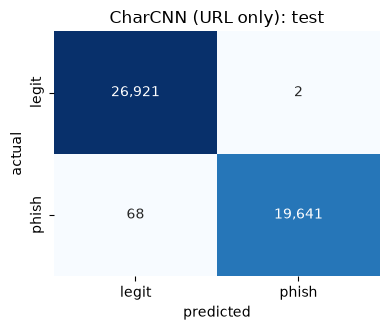
\includegraphics[width=0.5\linewidth]{figures/fig_charcnn_confusion.png}
\caption{CharCNN confusion matrix on the 46{,}632-row test set: 1 false
positive and 69 false negatives at threshold 0.5.}
\label{fig:charcnn-confusion}
\end{figure}

The URL-only model does not come in harder than the tabular models. It
essentially ties them and lands above the URL-only lexical literature
(\textcite{sahingoz2019}: 97.98\%; the char-CNN band in the SOTA
comparison: 97--99\%). So PhiUSIIL's separability is not confined to the
page-content columns Notebook 01 flagged; it is present in the raw URL
strings themselves. Legitimate and phishing URLs here come from
systematically different sources (well-known registrable domains versus
IP-address hosts, IPFS gateways, PaaS subdomains, randomized tokens),
differences visible character by character. This is the project's own
evidence for the benchmark-leakage critique in the SOTA comparison
(\cite{dalton2025}; \cite{das2019sok}).

Two caveats apply to the SOTA table. First, this model beats the URL-only
literature because PhiUSIIL is more separable than the cross-source
corpora those papers used, not because the architecture is stronger; the
claim is ``about 99.85\% on PhiUSIIL,'' not a general result. Second, the
exact-\code{Domain} split still lets registered-domain siblings on shared
platforms (\code{web.app}, \code{firebaseapp.com}, \code{repl.co}) fall on
both sides, which a character model could exploit as platform-level
memorization. The grouping analysis showed the tabular score is
near-invariant to this (0.9993 PaaS-aware versus 0.9995 exact), so it is
unlikely to be the main driver, but the CNN is more exposed to it than
logistic regression.

\subsection{Clustering: Phishing Attack Families}

The models so far are supervised. This section adds an unsupervised method,
the project's second algorithm type, and asks a different question: not
whether a URL is phishing, but what kinds of phishing are in the data. The
notebook clusters the phishing rows only on Notebook 01's leakage-clean
feature set (label held out) and profiles the groups as attack
``families.'' This is standard in the phishing literature
(\cite{feng2022} clustered phishing kits; \cite{althobaiti2023} clustered
campaigns; \cite{zia2025} clustered lexical URL tokens). Cluster IDs are
not fed back into the classifier, to avoid a second leakage-review cycle.
The method is KMeans with $k$ chosen by elbow and silhouette, centroid
profiling to name the families, PCA for a 2-D view, and HDBSCAN as a
density-based cross-check.

\subsubsection{Choosing \texorpdfstring{$k$}{k}}

The elbow and silhouette scans over $k$ appear in
Figure~\ref{fig:kmeans-selection} and Table~\ref{tab:kselect}. Here $k=2$
has by far the highest silhouette (0.44): the strongest structure is a
single binary split, matching Notebook 01's finding that phishing pages
divide into content-less shells versus content-bearing pages. The elbow is
otherwise soft, typical of high-dimensional tabular data with correlated
features. Because $k=2$ is too coarse for a families deliverable, the
notebook uses $k=5$, the silhouette peak among $k \geq 3$ and where the
elbow flattens. It reports the $k=2$ split as the dominant coarse
structure and profiles $k=5$ as interpretable strata. The silhouettes at
$k=5$ (about 0.15) are low, so these are overlapping descriptive families
rather than crisply separated clusters; HDBSCAN checks how much crisp
density structure exists.

\begin{table}[htbp]
\centering
\caption{KMeans model-selection scan over $k$ (silhouette on a 10k
sample).}
\label{tab:kselect}
\begin{tabular}{lcc}
\toprule
$k$ & Inertia & Silhouette (10k) \\
\midrule
2      & 4{,}500{,}166 & 0.437 \\
3      & 4{,}248{,}341 & 0.130 \\
4      & 3{,}923{,}595 & 0.149 \\
5      & 3{,}736{,}818 & 0.154 \\
6--10  & 3.58M--3.07M  & 0.089--0.121 \\
\bottomrule
\end{tabular}
\end{table}

\begin{figure}[htbp]
\centering
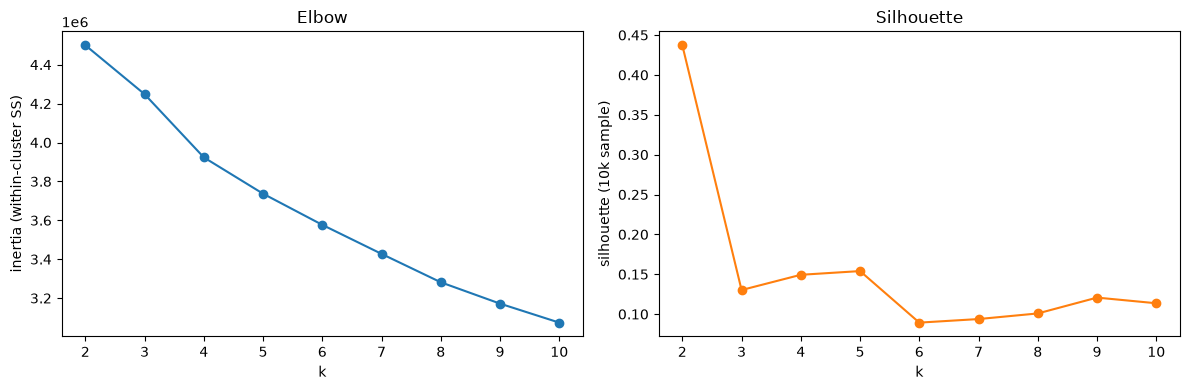
\includegraphics[width=0.9\linewidth]{figures/fig_kmeans_selection.png}
\caption{Elbow (inertia) and silhouette curves for KMeans. The silhouette
peaks sharply at $k=2$; $k=5$ is the local peak used for interpretable
families.}
\label{fig:kmeans-selection}
\end{figure}

\subsubsection{The Five Families}

Each cluster's raw-unit means and its centroid's top distinguishing
features (in standard deviations from the phishing-wide mean) give the
families in Table~\ref{tab:families}. Empty-shell pages dominate at 68\%,
consistent with Notebook 01's finding that most phishing rows are
content-less and with the $k=2$ super-split (87/13) that separates these
from content-bearing pages. The two active attack types separate cleanly:
credential-harvesting forms (c3), with the password/submit/hidden-field
signature of a fake login, and HTTP lookalike stubs (c4), which look
brand-consistent but lack HTTPS. Cluster c1 holds only 5 rows; KMeans
minimizes squared distance and is sensitive to outliers, so a few
4{,}000-character URLs captured their own centroid. This is a KMeans
artifact, not a real family, and the HDBSCAN cross-check relabels these as
noise.

\begin{table}[htbp]
\centering
\caption{The five phishing families from KMeans ($k=5$).}
\label{tab:families}
\footnotesize
\setlength{\tabcolsep}{4pt}
\begin{tabularx}{\linewidth}{>{\raggedright\arraybackslash}p{2.7cm}>{\raggedright\arraybackslash}p{3.1cm}Y}
\toprule
Cluster (size) & Attack family & Defining signature \\
\midrule
c0 -- 68{,}743 (68.4\%) & Empty-shell pages &
  No title, no forms, about 40 lines of code, low title-match
  (parked/stub, no real content) \\
c3 -- 11{,}809 (11.7\%) & Credential-harvesting forms &
  Password, submit, hidden fields, images, CSS, favicon, about 267 lines
  of code (fake logins) \\
c4 -- 18{,}830 (18.7\%) & HTTP lookalike stubs &
  Title matches domain, short clean URLs, only 17\% HTTPS
  (brand-consistent, plain HTTP) \\
c2 -- 1{,}133 (1.1\%) & IP-host / obfuscated pages &
  \code{HasObfuscation}, 39\% IP-hosted, long URLs, many \code{?} params \\
c1 -- 5 (0.0\%) & Outlier micro-cluster &
  URL length about 4{,}128 chars, extreme obfuscated/digit/ampersand
  counts (ultra-long parameter-stuffed URLs) \\
\bottomrule
\end{tabularx}
\end{table}

\subsubsection{What the Clustering Shows}

KMeans ($k=5$) partitions phishing into interpretable strata: one dominant
empty-shell family (68\%) and two distinct active types,
credential-harvesting forms (12\%, password/submit/hidden-field signature)
and HTTP lookalike stubs (19\%, domain-matching titles but no HTTPS), plus
a small IP-host / obfuscated-URL group (1\%) and a 5-row outlier artifact.
This mirrors the supervised EDA in Notebook 01: most phishing pages are
content-less shells, and the rest split into ``steal credentials
directly'' versus ``look legitimate cheaply''
(Figure~\ref{fig:pca-families}).

\begin{figure}[htbp]
\centering
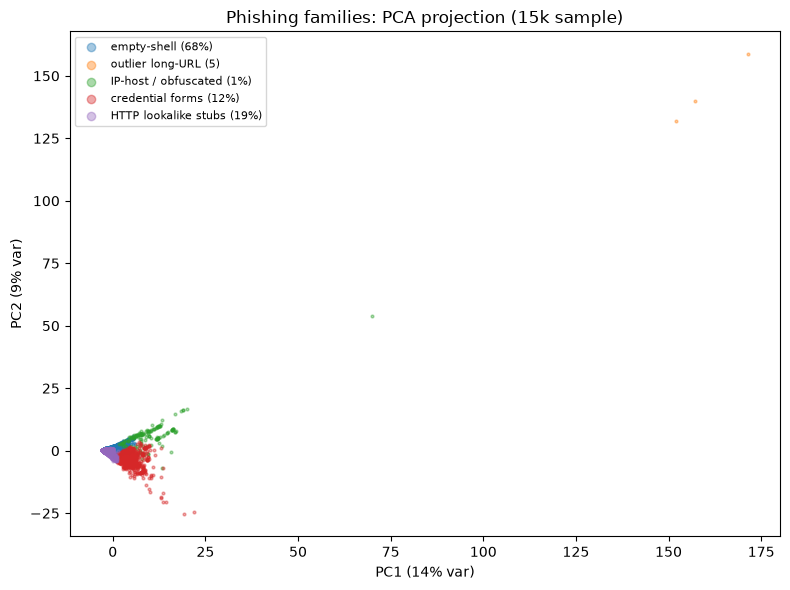
\includegraphics[width=0.7\linewidth]{figures/fig_pca_families.png}
\caption{PCA projection of the phishing families (15k sample). The
projection is one dense overlapping mass with a few outlier spikes rather
than five separated islands; the first two components explain 22.9\% of
variance.}
\label{fig:pca-families}
\end{figure}

The structure is soft. Three signals say these are convenient strata over
a partly continuous space rather than sharply separated kinds. First,
silhouettes are low (about 0.15 at $k=5$; only the $k=2$ empty-versus-
content split scores well, at 0.44). Second, PCA is diffuse: the first two
components explain 22.9\% of variance, and the projection is one dense
overlapping mass with a few outlier spikes (the 5 long-URL points, one
IP-host page, the credential-form tail), not five islands. Third, HDBSCAN
found 25 micro-clusters and left 30\% as noise on a 25k sample, rather
than five clean families. The micro-clusters likely correspond to
near-identical phishing kits (templated pages reused across many URLs),
the finer level \textcite{feng2022} found; the 30\% is genuinely
continuous. The 5-row KMeans outlier does not survive as an HDBSCAN
cluster, confirming it was an artifact. So KMeans $k=5$ is the descriptive
lens that names recognizable attack families and ties them to the
supervised findings, while HDBSCAN is the validity check showing the true
structure is a few dominant modes plus many small kit-level pockets and a
continuous remainder. The contrast between partition-based and
density-based clustering is itself a result for the write-up.

\subsection{State-of-the-Art Comparison}

Two framing rules govern the comparison. First, numbers are comparable
only within a dataset; accuracy on PhiUSIIL and accuracy on another corpus
are different measurements, so the CharCNN's about 99.85\% is on PhiUSIIL,
directly comparable to other PhiUSIIL numbers and only contextually
comparable to URL-only models on other corpora. Second, published numbers
are flagged by verification status: several come from secondary citations
because the primary papers were not directly accessible, and sources
sometimes disagree, so those are marked unverified and treated as
directional. Figure~\ref{fig:sota-bar} places the project's supervised
models against the published PhiUSIIL band.

\begin{figure}[htbp]
\centering
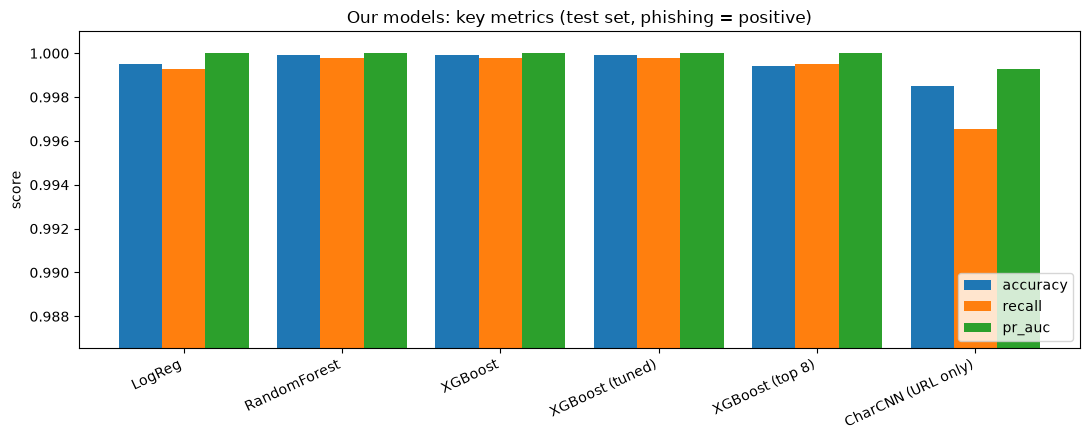
\includegraphics[width=0.9\linewidth]{figures/fig_sota_bar.png}
\caption{The project's models against the published PhiUSIIL 99.5--100\%
band. All five supervised models fall inside the band; the CharCNN is the
informative near-tie.}
\label{fig:sota-bar}
\end{figure}

\subsubsection{Published Results in Context}

Table~\ref{tab:sota-phiusiil} lists results on the same dataset (PhiUSIIL),
directly comparable to the project's rows, and Table~\ref{tab:sota-urlonly}
lists URL-only and lexical results on other datasets, included for context
only.

\begin{table}[htbp]
\centering
\caption{Published results on PhiUSIIL, with the project's own rows.}
\label{tab:sota-phiusiil}
\footnotesize
\setlength{\tabcolsep}{4pt}
\begin{tabularx}{\linewidth}{Y>{\raggedright\arraybackslash}p{2.9cm}Y}
\toprule
Study & Approach & Reported / status \\
\midrule
\textcite{prasad2024phiusiil} (dataset authors) &
  similarity-index + incremental learning &
  $\sim$99.2--99.8\% (one source 99.97\%); unverified, sources disagree \\
\textcite{pentapalli2025} &
  TSK fuzzy; excluded \code{URLSimilarityIndex} &
  qualitative agreement with our leakage call \\
Independent reproductions (Kaggle, small papers) &
  RF / DT / KNN / LR / XGB / FCNN / BERT &
  99.5--100\% band; aggregated, unverified \\
This project, tuned XGBoost (NB 02) & full leakage-clean feature set &
  see Table~\ref{tab:topk} \\
This project, CharCNN (URL only) & raw URL characters only &
  0.9985 acc / 0.9993 PR-AUC \\
\bottomrule
\end{tabularx}
\end{table}

\begin{table}[htbp]
\centering
\caption{URL-only / lexical literature on other datasets (context only).}
\label{tab:sota-urlonly}
\footnotesize
\setlength{\tabcolsep}{4pt}
\begin{tabularx}{\linewidth}{Y>{\raggedright\arraybackslash}p{2.5cm}cY}
\toprule
Study & Approach & Reported acc & Status \\
\midrule
\textcite{sahingoz2019} & RF on 39 NLP lexical features & 97.98\% &
  corroborated; firmest external number \\
\textcite{yerima2020} & char-CNN & 98.2\% (F1 0.976) & reported (arXiv) \\
\textcite{maneriker2021urltran} (URLTran) & BERT on subword URLs &
  about 96\% & reported (arXiv) \\
\textcite{minilm2024} & MiniLM-CNN-LSTM hybrid & 98.98\% & reported \\
\textcite{dubey2025} & char-CNN + LightGBM & 99.82\% & reported (arXiv) \\
\textcite{mohammad2014} & self-structuring NN & 92--96\% (disputed) &
  unverified; hedge or drop \\
\bottomrule
\end{tabularx}
\end{table}

These bracket a 97--99\% range for URL-only models on harder cross-source
corpora. The CharCNN lands above that band because PhiUSIIL is more
separable at the raw-string level, not because the architecture is
stronger. Precedents for the other methods: for the imbalance ablation,
\textcite{omari2025} report SMOTE-NC + XGBoost at 98.0\% precision /
98.5\% recall; for the clustering, \textcite{feng2022} (k-medoid on
phishing kits, 90.1\% TPR) and \textcite{zia2025} (LSH on lexical tokens,
93\% on PhishStorm) frame attack-family clustering as standard practice.

\subsubsection{Where Our Results Land}

Against PhiUSIIL, every one of the project's models sits in the published
99.5--100\% band: logistic regression 0.9995, random forest 0.9999,
XGBoost 1.0000, tuned XGBoost 0.9999, and a top-8-feature model at 0.9993.
This reproduces the dataset authors' range and the independent
reproductions across model families; it confirms a known ceiling rather
than producing an outlier. At four decimals almost everything rounds to
about 1.0, so accuracy ordering is noise. The informative comparison is
the CharCNN: 0.9985 accuracy and 0.9993 PR-AUC on the same 46{,}632-row
test split, within 0.0015 accuracy of the full-feature XGBoost. A model
denied \code{URLSimilarityIndex}, the page-content flags, and the
engineered features, seeing only the raw URL string, matches models that
see all 49 clean features. That is direct evidence from the project's own
pipeline that PhiUSIIL's separability is in the URL strings, not just the
content columns Notebook 01 flagged, and it corroborates the
benchmark-leakage critique rather than only citing it. The supervised
problem is saturated; the useful question is why. The contribution of this
notebook is not a new ceiling number but the leakage-immune CharCNN and
the clustering, which together characterize what makes the benchmark easy
and what kinds of phishing it contains.

% =====================================================================
\section{Synthesis and Discussion}
% (Written for the report; minimal, ties everything together.)
% =====================================================================

The three notebooks converge on one claim: on PhiUSIIL, the separability
of phishing from legitimate URLs is intrinsic to the data, not an artifact
of a single leaky column or a favorable split. The project demonstrates
this three separate ways. The data audit showed that removing the obvious
leak, \code{URLSimilarityIndex}, leaves the remaining features at about
99.9\%. The grouping analysis showed that tightening the train/test split
from exact-domain to registered-domain grouping, across a range of more
than 44{,}000 groups, moves accuracy only from 0.9995 to 0.9990. And the
character model, which sees nothing but the raw URL string and therefore
cannot leak, still reached 0.9985 accuracy. Three different attempts to
make the problem harder all failed to move the number in any meaningful
way. That consistency is the result.

The project also satisfies the course requirement to combine at least two
algorithm families under experimental comparison. It uses supervised
classification (logistic regression, random forest, and XGBoost) and
unsupervised clustering (KMeans and HDBSCAN), and it runs several
controlled comparisons within those: an imbalance ablation
(none versus class weighting versus SMOTE), hyperparameter tuning with
grouped cross-validation, a full-model versus top-8-feature comparison, a
partition-based versus density-based clustering cross-check, and a
character-level model set against both the tabular models and the
published literature. The empirical comparisons are presented graphically
where possible, as the assignment prefers.

Two things are worth stating about what the project does and does not
claim. It does claim that PhiUSIIL is easy for reasons that go all the way
down to the raw URL characters, and that the easy-benchmark result should
be read as evidence about the dataset rather than about any one model. It
does not claim a general phishing-detection breakthrough. The character
model beats the URL-only literature because PhiUSIIL is more separable than
the cross-source corpora those studies used, not because the architecture
is stronger. The honest phrasing is ``about 99.85\% on PhiUSIIL,'' full
stop.

A consistent caveat runs through the state-of-the-art comparison: many of
the published numbers are vendor-reported or come from secondary citations
that were not independently verified, and sources sometimes disagree.
Those numbers are treated as directional rather than exact, and the tables
flag their verification status. The safest reading of the comparison is
that the project's results reproduce a known ceiling, not that any single
external figure is authoritative.

The main limitations follow from the benchmark itself. Because PhiUSIIL is
so separable, the accuracy ordering among models is noise, so the useful
work shifted to interpretation: the cost-sensitive operating points, the
feature-importance finding that a handful of features suffices, and the
clustering that names attack families. The exact-domain split also leaves
platform-level siblings on shared hosting on both sides of the split,
which the character model is more exposed to than the linear model; the
grouping analysis suggests this is not the main driver, but a fully
platform-aware split would close the gap. Natural next steps are to test
the trained models on a different corpus to measure how much of the
performance is PhiUSIIL-specific, and to feed the kit-level structure that
HDBSCAN surfaced into a more operational grouping of phishing campaigns.

% =====================================================================
\section{Conclusion}
% =====================================================================

This project built and compared a full phishing-URL detection pipeline on
PhiUSIIL: a leakage audit and exploratory analysis, three classical
classifiers with imbalance, tuning, feature-importance and cost-sensitive
analyses, a character-level convolutional model on the raw URL string, and
an unsupervised clustering of phishing into attack families. Every
supervised model landed in the published 99.5--100\% band, and the
leakage-immune character model essentially tied them. The contribution is
not a new accuracy number but an explanation of why the benchmark is easy,
established from three independent directions, together with a
characterization of the kinds of phishing the dataset contains. The result
is a report that treats near-perfect accuracy as something to be
explained rather than celebrated.

% =====================================================================
\printbibliography
% =====================================================================

% =====================================================================
\appendix

\section{Contribution Statement}
% NOTE: confirm/adjust these with the team before submission.

The project was divided by notebook, with each member owning one notebook
end to end and the report assembled collaboratively.

\begin{itemize}
  \item \textbf{Guna Pasupathy} authored Notebook 01 (data loading, the
    three-part leakage audit, exploratory data analysis, and the saved
    leakage-clean feature manifest that the other notebooks consume).
  \item \textbf{Jason Justice} authored Notebook 02 (feature engineering
    from the raw URL/Domain strings, the three classical classifiers, the
    class-imbalance ablation, hyperparameter tuning, feature-importance
    analysis, the top-8-feature comparison, and the cost-sensitive
    decision layer).
  \item \textbf{Pranav Dhinakar} authored Notebook 03 (the
    registered-domain grouping decision, the character-level CNN on raw
    URLs, the KMeans/HDBSCAN clustering of attack families, and the
    state-of-the-art comparison) and assembled this report.
\end{itemize}

\emph{[Team: confirm the exact split of report writing, presentation, and
repository maintenance here before submission.]}

\section{Generative-AI Use Disclosure}
% NOTE: edit to reflect actual usage before submission.

Consistent with the course policy, the team discloses its use of
generative-AI tools. All modeling code, experimental design, analysis, and
numerical results in the three notebooks are the team's own work. A
large-language-model assistant was used to help assemble and format this
LaTeX report from the notebooks' existing author-written markdown notes,
to convert notebook tables and figures into report tables and captions,
and to draft the introduction, synthesis, and conclusion sections, which
were then reviewed and edited by the authors. The assistant did not
generate the analysis or the results. Any AI-assisted passages were
checked against the notebook outputs for accuracy. \emph{[Team: add any
other tools used during development, for example code assistance in the
notebooks, and adjust this statement to match.]}

\section{Source Code}

The complete, documented source code for the three notebooks is listed
below, exported from the committed Jupyter notebooks. The authoritative
version, with full commit history and outputs, is in the team GitHub
repository linked on the title page.

\singlespacing

\subsection{Notebook 01 -- Load, Leakage, EDA (Guna Pasupathy)}
\lstinputlisting[style=py]{source_code/nb01.py}

\subsection{Notebook 02 -- Classical Models (Jason Justice)}
\lstinputlisting[style=py]{source_code/nb02.py}

\subsection{Notebook 03 -- CharCNN, Clustering, SOTA (Pranav Dhinakar)}
\lstinputlisting[style=py]{source_code/nb03.py}

\end{document}
